\documentclass{article}
\usepackage[utf8]{inputenc}

%\usepackage[md]{titlesec}
\usepackage{graphicx}

\usepackage[export]{adjustbox}

\usepackage{subcaption}

\setcounter{tocdepth}{1}

\renewcommand{\thesubsection}{\alph{subsection}}
%\renewcommand{\thesubsubsection}{\arabic{\subsubsection}}



\date{October 14, 2016}


\title{\textbf{Assignment 7}\\Packet Tracer}
\author{s316620}


\begin{document}



\maketitle

\newpage

\tableofcontents

\newpage
\part{Introduction}

The goal of this assignment is to get familiar with Packet Tracer, practice configuration and compare with previous works, Openvswitch and Quagga. Packet Tracer is a virtual network simulator developed by Cisco.

\part{Materials and Methods}


\section{Console access to a router in the real world (emulated in PacketTracer)}

\subsection{Setting up the Router and Host}
First we setup a connection between a Router and a host. Open Packet Tracer and add a Router and a host, then connect the two using a cable. The router used in my setup was \textit{router 1841} and a \textit{generic host}. The cable was connected on the router on the \textit{console port} and the \textit{RS-232 port} on the host/PC. The setup can be seen in the Figure \ref{fig:firstset}.
\begin{figure}[h]
    \centering
    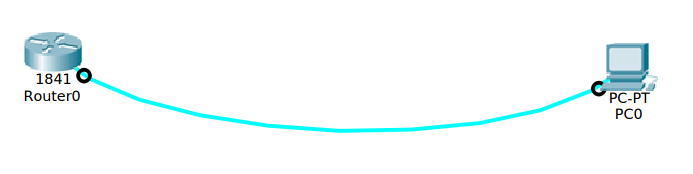
\includegraphics[width=\textwidth]{firstsetup}
    \caption{Initial Setup}
    \label{fig:firstset}
\end{figure}

\subsection{Accessing the router's CLI}
To access the Command Line Interface (CLI) of the router, click on the PC0 in Packet Tracer. Select the 'Desktop' tab, and double-click on the 'Terminal' window. The default 'Terminal Configuration' is left unchanged. After clicking 'OK' we can see the router's CLI. The CLI asks to continue with the initial configuration dialog. The answer is 'no' in all the configuration throughout the assignment. The we start with the CLI in the user exec mode. 

\subsection{Command modes}
When the router starts we get the prompt '\textit{Router\textgreater}', this shows that we are in the User EXEC mode ("user mode"). To change into the Privileged EXEC mode we can issue the command \textbf{enable}, similarly we can go back to the user exec mode by running the command \textbf{disable}. The prompt changes when in the Privileged exec mode to : \textit{Router\#}. To go from the privileged exec mode to the configuration mode we can use the command \textbf{configure terminal},(\textit{\textbf{config term} or \textbf{conf t}}) is the shortcut. When in the config mode the prompt changes to : \textit{Router(config)\#}. The different command modes limits the different commands the user can input. We can check the commands available in each mode by running the command '\textbf{?}'.

\subsection{The \textit{show} and the \textit{do} commands.}
The \textbf{show} command has a lot of different options, it can be used with. This commands lists the specified options. The \textbf{show startup-config} command shows the start up configuration of the device. In our case nothing is shown as no startup configuration is set. The \textbf{show running-config} command shows the running configuration. We can see some configuration when we run this. The \textbf{show} command is run in the Privileged exec mode (enable mode). If in the config mode and we want to run the command available only in the enable mode, we can use the command \textbf{do} as a prefix ot the command we want to run. For example, if in the config mode and we run the command \textbf{do show running-config} we can see the running configuration without having to go to the enable mode.

\subsection{Changing hostname}
We can change the hostname of the device, by executing the command \textbf{hostname MyRouter} in the config mode. We can see the changes in the running-config, but not in the startup-config.

\subsection{Rebooting the device}
We can use the command \textbf{reload} to reboot the device. After reboot the hostname changes back to the default name 'Router'. This is because there was no startup-config, every time the machine reboots it applies the startup-config if any while it discards the running-config at shutdown. 

\subsection{Making persistent changes}
To save changes persistently even after reboots, we need to save it in the startup-config. There are two commands to do this, the \textbf{copy running-config startup-config} command copies the running-config into startup-config or the command \textbf{write}, which is executed in the enable mode. 

\subsection{Checking the current version}
We can use the \textbf{show version} command to see the Cisco IOS software version along with other information. Our router is running the 1841 Software with version 12.4(15)T1, as seen in Figure \ref{fig:rver}. 

\begin{figure}[h]
    \centering
    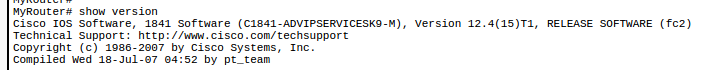
\includegraphics[width=\textwidth]{routerver}
    \caption{Running the \textit{show version} command.}
    \label{fig:rver}
\end{figure}


\section{Connecting two hosts to a router in PacketTracer}

\subsection{Setting up the hosts in Packet Tracer}

\begin{figure}[h]
    \centering
    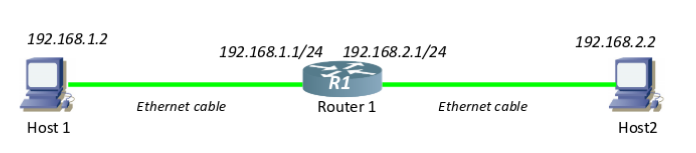
\includegraphics[width=\textwidth]{2top}
    \caption{Topology from Figure 2 in Assignment 7}
    \label{fig:2top}
\end{figure}

We set up the two hosts connected to a router as instructed in the assignment, the topology can be seen in Figure \ref{fig:2top}. Setting this up in Packet Tracer we use two generic hosts and one 1841 router, the connection is made using the copper crossover cable. The setup in the Packet Tracer can be seen in Figure \ref{fig:2toppt}. The IP addresses on Host1 and Host2 are 192.168.1.2/24 and 192.168.2.2/24. The router has the IP address 192.168.1.1/24 on port FastEthernet0/0 and the IP address 192.168.2.2/24 on the port FastEthernet0/1. The default gateway for Host1 is 192.168.1.1 and the default gateway for Host2 is 192.168.2.2.

\begin{figure}[h]
    \centering
    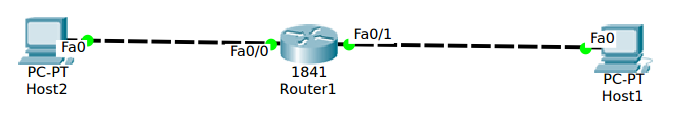
\includegraphics[width=\textwidth]{pt2set}
    \caption{Topology in Packet Tracer}
    \label{fig:2toppt}
\end{figure}


The configuration of the IP address on the hosts can be done by clicking on the host, this opens a window, then goto the "Config" tab, in the "INTERFACE-{\textgreater}FastEthernet" menu, we can edit the IP address. Similary the Gateway IP address can be configure in the "GLOBAL-{\textgreater}Settings" menu. This method was used to configure Host1 and can be seen in Figure \ref{fig:host1config}. 

\begin{figure}[h]
    \centering
    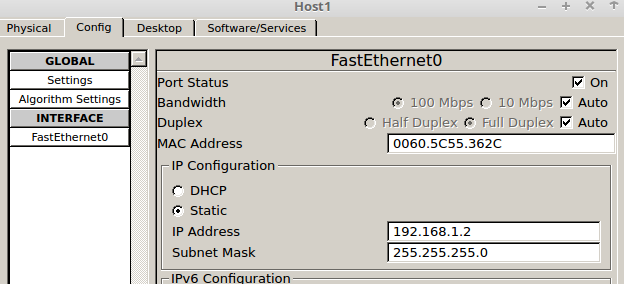
\includegraphics[width=\textwidth]{host1inter}
    \vspace{0.8cm}
    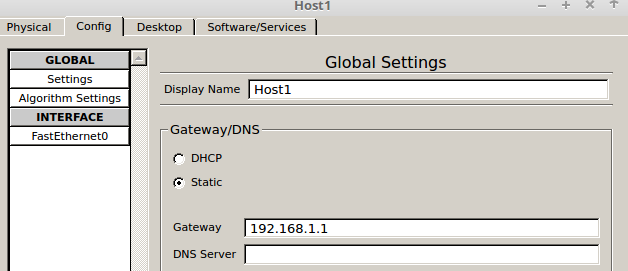
\includegraphics[width=\textwidth]{host1gate}
    \caption{Configuring the IP address and the default Gateway for Host1.}
    \label{fig:host1config}
\end{figure}

The Host2 was configured by clicking on the host and then going to the "Desktop" tab, then clicking on "IP Configuration". The we can set the configurations as seen in Figure \ref{fig:host2config}.
\begin{figure}[!h]
    \centering
    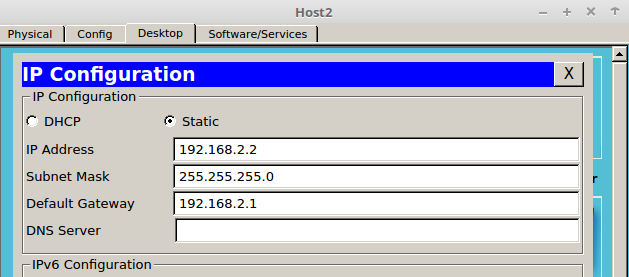
\includegraphics[width=\textwidth]{host2config}
    \caption{Host2 IP address and default Gateway Cofiguration}
    \label{fig:host2config}
\end{figure}
\newpage
\subsection{Configuring the Router}

To configure the router click the router and go to the "CLI" tab. From the command line interface (CLI), we can configure the router as seen in Figure \ref{fig:2routerconfig}. The configuration is done in the \textit{config mode}. 

\begin{figure}[h]
    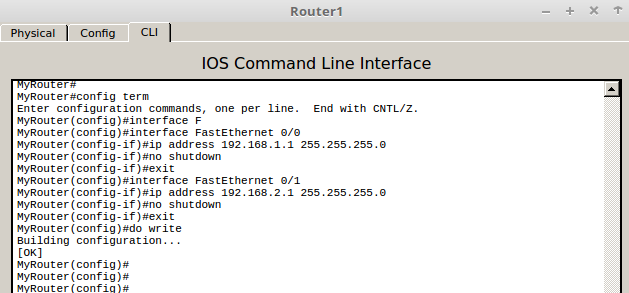
\includegraphics[width=\textwidth]{2routerconf}
    \caption{Configuring the Router IP addresses}
    \label{fig:2routerconfig}
\end{figure}

\newpage
\subsection{Reachability test}

We can check the reachability between the three nodes using the \textbf{ping} command. We can see Figure \ref{fig:pinghosts} to see that all the hosts are reachable, we ping all the interfaces from Host2. 

\begin{figure}[h]
    \centering
    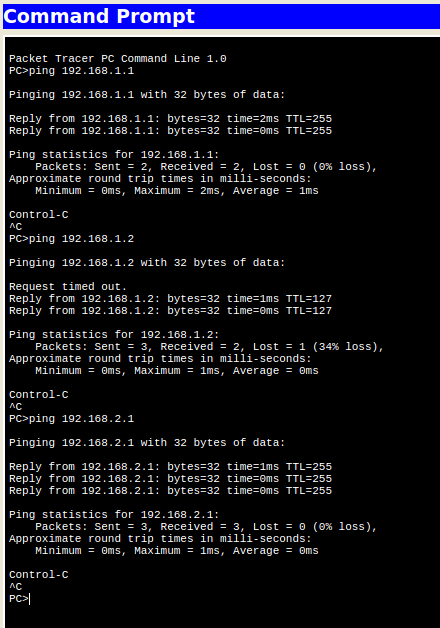
\includegraphics[width=0.6\textwidth]{2pinghosts}
    \caption{Checking connectivity of all the hosts using the \textit{ping} command from Host2.}
    \label{fig:pinghosts}
\end{figure}

\newpage
\subsection{Statistics for all the interfaces}

The \textbf{show interfaces} command is executed in the \textit{enable mode}, it shows the statistics for all the interfaces on the router, as seen in Figure \ref{fig:2routerstat}. 

\begin{figure}[!h]
\centering
    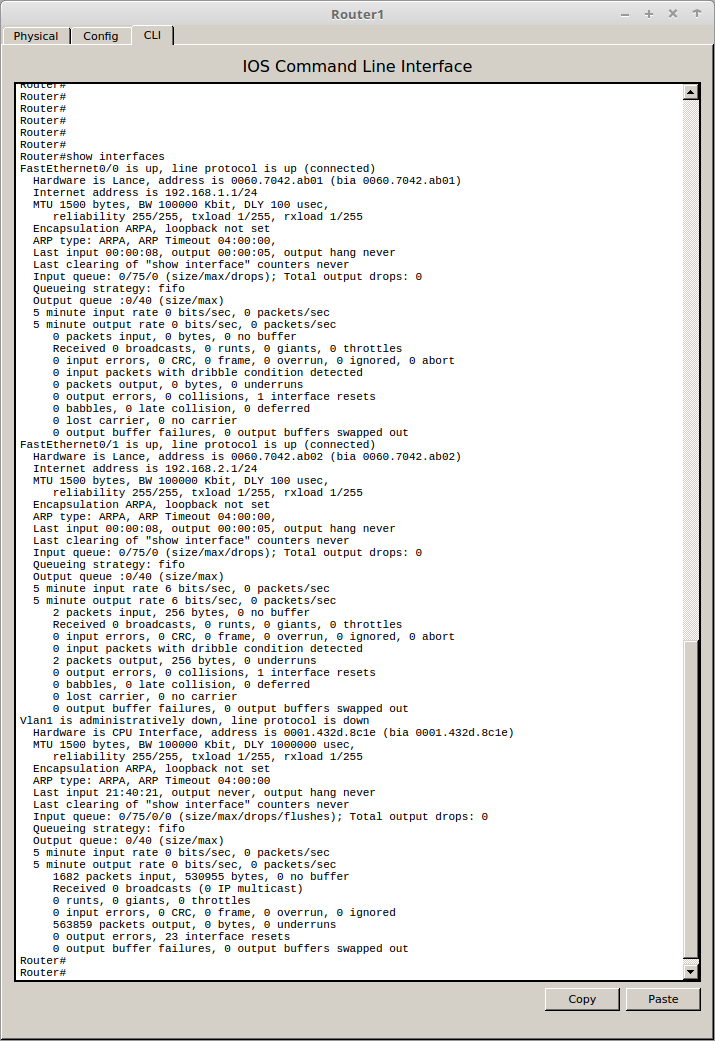
\includegraphics[scale=0.4]{2routerstat}
    \caption{Running the \textit{show interfaces} command at Router1.}
    \label{fig:2routerstat}
\end{figure}


\subsection{Display flash memory information}

The \textbf{show version} command can be used to see the flash memory information as seen in Figure \ref{fig:2routermem}. 
\begin{figure}[h]
\centering
    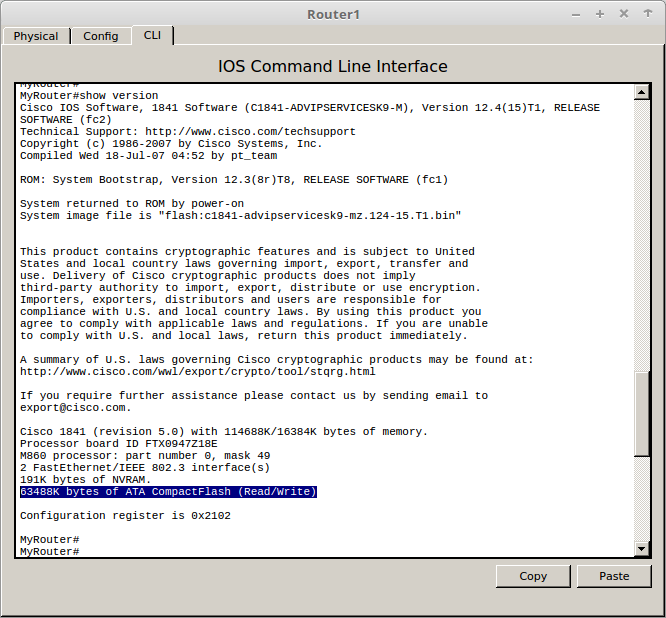
\includegraphics[scale=0.4]{2routermem}
    \caption{Running the \textit{show version} command at Router1.}
    \label{fig:2routermem}
\end{figure}


\section{Static routing configuration in PacketTracer}


\begin{figure}[h]
    \centering
    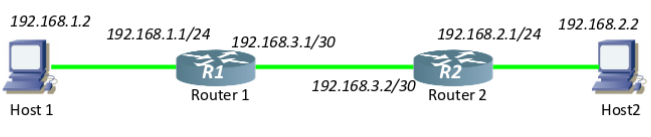
\includegraphics[width=\textwidth]{3top}
    \caption{Assignment 7 Figure 3 topology}
    \label{fig:3top}
\end{figure}

\subsection{Adding another router to the setup}

Now modifying the current topology to look like Figure \ref{fig:3top}. Implementing this, the new topology in Packet Tracer is shown in Figure \ref{fig:3pttop}. 

\begin{figure}[h]
    \centering
    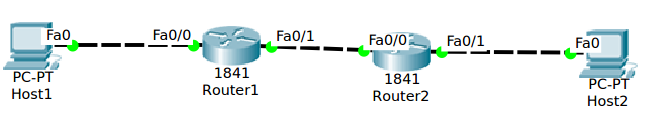
\includegraphics[width=\textwidth]{3pttop}
    \caption{Packet Tracer topology with two routers.}
    \label{fig:3pttop}
\end{figure}

We need to configure static routing in the routers for reachability between the networks the two hosts are in, we do this in the "CLI" of each of the routers as seen in Figure \ref{fig:3routersconf}.

\begin{figure}[h]
\begin{subfigure}{0.5\textwidth}
    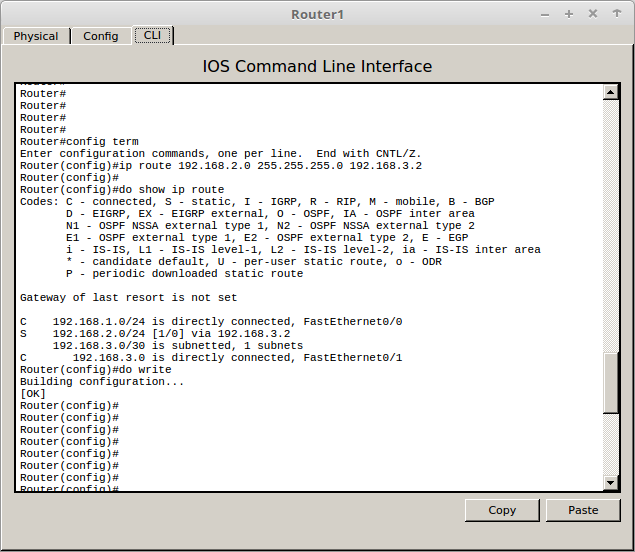
\includegraphics[width=\linewidth]{3routersconf1}
    \caption{Configuring static routing for the router 1}
    \label{fig:3routersconf1}
\end{subfigure}
%
\begin{subfigure}{0.5\textwidth}
    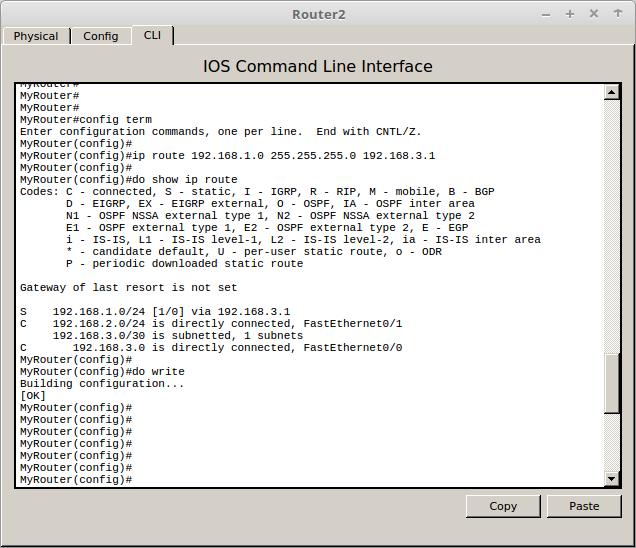
\includegraphics[width=\linewidth]{3routersconf2}
    \caption{Configuring static routing for the router 2}
    \label{fig:3routersconf2}
\end{subfigure}

 \caption{Configuring static routing for the routers}
    \label{fig:3routersconf}
\end{figure}


As seen in Figure \ref{fig:3ping} we can see that all hosts are reachable from each other. Configuring this in PacketTracer compared to Quagga was a few commands, in Quagga we could use the command \textbf{ip address {\textless}\textit{IP address/24}{\textgreater}} to define the 255.255.255.0 subnet but in PacketTracer we have to explicitly specify it, like \textbf{ip address {\textless}\textit{IP address}{\textgreater} 255.255.255.0}. That was the only difference I noticed.

\begin{figure}[h]
    \centering
    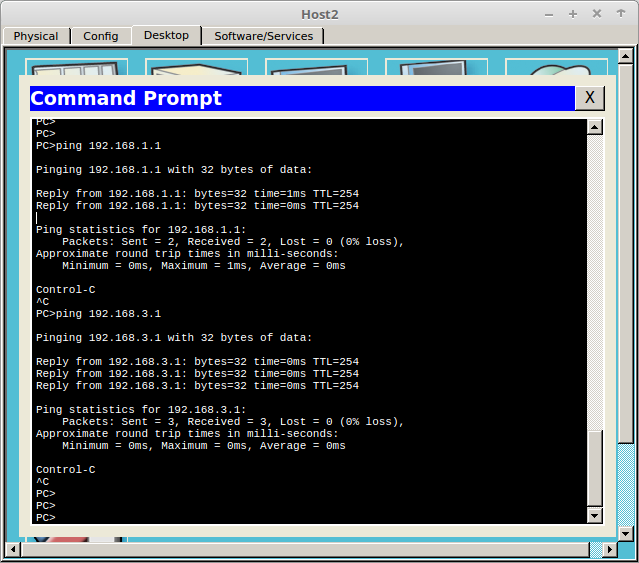
\includegraphics[scale=0.4]{3ping}
    \caption{Using ping to check connectivity between hosts from Figure \ref{fig:3pttop} topology.}
    \label{fig:3ping}
\end{figure}



\section{More static routing in Packet Tracer}

\begin{figure}[h]
    \centering
    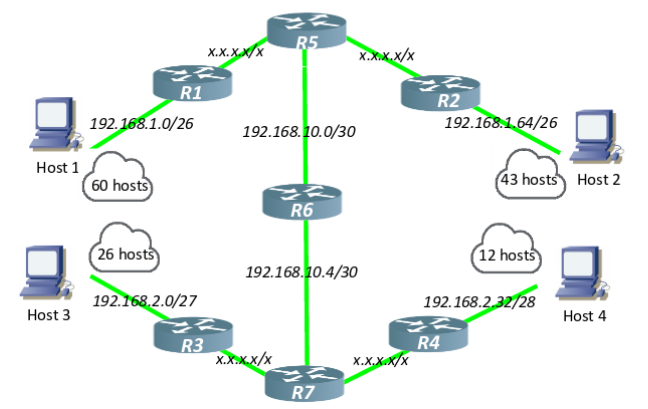
\includegraphics[scale=0.3]{4topassign}
    \caption{Network topology for Figure 4 from Assignment 7}
    \label{fig:4topassign}
\end{figure}

\begin{figure}[h]
    \centering
    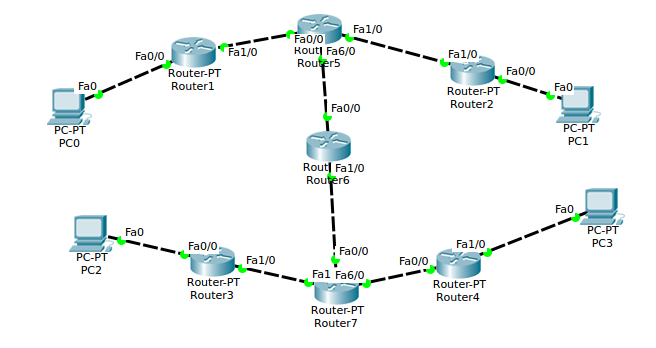
\includegraphics[scale=0.3]{4toppt}
    \caption{Network topology for Figure 4 from Assignment 7}
    \label{fig:4toppt}
\end{figure}
Now we configure static routing as in the topology specified in the assignment as seen if Figure 
\ref{fig:4topassign}. The topology in Packet Tracer can be seen in Figure \ref{fig:4toppt}. All the routers used are generic, for Router5 and Router7 there are not enough interfaces so we click the routers, go to the "Physical" tab and add the "PT-Router-NM-1CFE" module. To add the modules the device should be powered off, if any changes have been made to the router it needs to be saved persistently with the \textbf{write} command in the \textit{enable mode}. 

\begin{table}[!h]
    \centering
    \begin{tabular}{c|c|c}
    \hline
        Device & Interface & IP address/subnet \\
        \hline
        Host1  & Fa0 &192.168.1.2/26 \\
        Host2 & Fa0 & 192.169.1.66/26 \\
        Router1 & Fa0/0 & 192.168.1.1/26 \\
        Router1 & Fa1/0 & 192.168.1.130/30 \\    
        Router2 & Fa0/0 & 192.168.1.65/26 \\
        Router2 & Fa1/0 & 192.168.1.134/30\\
        Router5 & Fa0/0 & 192.168.1.129/30 \\
        Router5 & Fa1/0 & 192.168.1.133/30 \\
        Router5 & Fa6/0 & 192.168.10.2/30 \\
        Router6 & Fa0/0 & 192.168.10.1/30 \\
        Router6 & Fa1/0 & 192.168.10.5/30 \\
        Router7 & Fa0/0 & 192.168.10.6/30 \\
        Router7 & Fa1/0 & 192.168.2.49/30 \\
        Router7 & Fa6/0 & 192.168.2.53/30 \\
        Router3 & Fa0/0 & 192.168.2.1/27 \\
        Router3 & Fa1/0 & 192.168.2.50/30 \\    
        Router4 & Fa0/0 & 192.168.2.54/30 \\
        Router4 & Fa1/0 & 192.168.2.33/28\\
        Host3  & Fa0 & 192.168.2.2/27 \\
        Host4 & Fa0 & 192.169.2.34/28 \\
        \hline
    \end{tabular}
    \caption{IP addresses for the interfaces of different devices for the topology in Figure \ref{fig:4topassign} and \ref{fig:4toppt} . }
    \label{tab:4ips}
\end{table}

We assign Routers and the hosts the IP addresses which can be seen in Table \ref{tab:4ips}. And use default gateways at the hosts and set up OSPF routing at the routers. The OSPF routing is setup in each router this was set up as seen in Figure \ref{fig:4ospfconf}. 

\begin{figure}[!h]
    \centering
    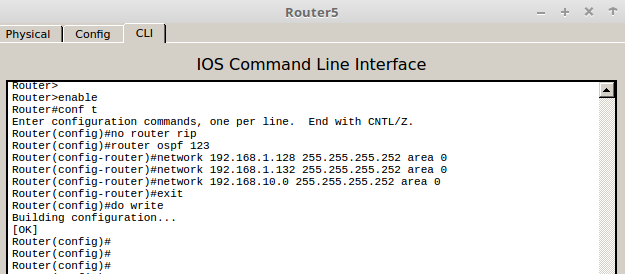
\includegraphics[width=\textwidth]{4ospfconf}
    \caption{Caption}
    \label{fig:4ospfconf}
\end{figure}

Then we can check the connectivity of the network by pinging the hosts from each other. I ping Host2, Host3 and Host4 from Host1 as seen in Figure \ref{fig:4pingcon}. We can see that all the pings return successfully. As the hosts have connection to each other the we can conclude that the routers are working correctly as well. 

\begin{figure}[h]
    \centering
    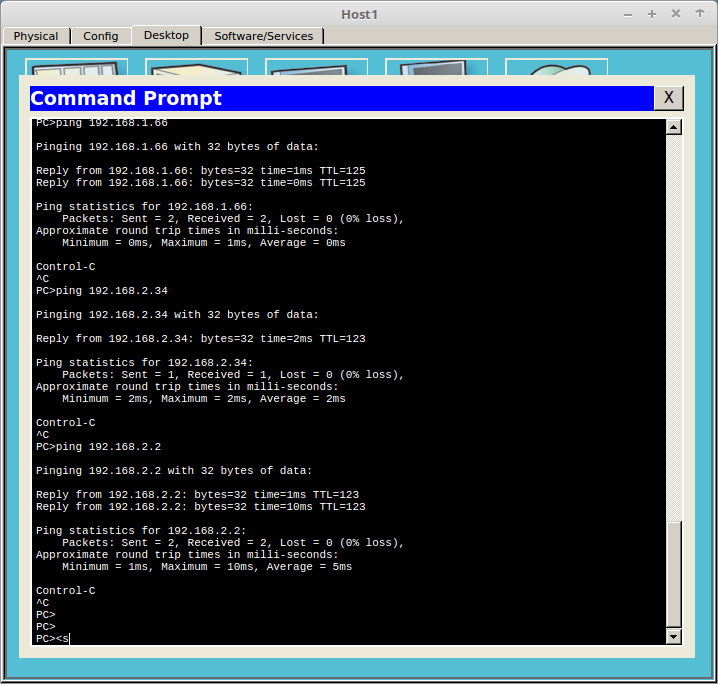
\includegraphics[width=0.7\textwidth]{4pingcon}
    \caption{Testing connectivity of the topolgy by pinging Host2, Host3 and Host4 from Host1.}
    \label{fig:4pingcon}
\end{figure}

\section{More static routing and RIP}

\subsection{Set up static routing}

We set up a new topology in Packet Tracer as seen in Figure \ref{fig:5toppt} and set up the IP addresses for routers and hosts as done in the previous assignment. PC1, PC2 and PC3 have the IP addresses 192.168.1.2, 192.168.1.66 and 192.168.1.130 respectively. And the routers have IP addresses as seen in Table \ref{tab:5routerip}. 

\begin{table}[]
    \centering
    \begin{tabular}{c|c|c}
    \hline
         Router & Interface & IP  \\
    \hline
         Router1 & Fa 0/0 &  192.168.1.1\\
         Router1 & Fa 0/1 & 10.0.0.2 \\
         Router2 & Fa 0/0 & 192.168.1.66\\
         Router2 & Fa 0/1 & 10.0.0.6 \\
         Router3 & Fa 0/0 & 10.0.0.10\\
         Router3 & Fa 0/1 & 192.168.1.129\\
         Router5 & Fa 0/0 & 10.0.0.1\\
         Router5 & Fa 0/1 & 10.0.0.5\\
         Router5 & Fa 1/0 & 10.0.0.9\\
         \hline
    \end{tabular}
    \caption{Caption}
    \label{tab:my_label}
\end{table}

Then configuring the routes for the hosts and the routers, all the hosts have default gateway to the IP address of the interface of the router they are connected to and Router1, Router2 and Router3 have Router5 as their default Gateway. This was done as seen in Figure \ref{fig:5routerdefgw} for all the routers with the gateway as Router5
s interface. For Router5 we added the static routes to the networks as seen in \ref{fig:5router5def}.

\begin{figure}[h]

\begin{subfigure}{0.5\textwidth}
       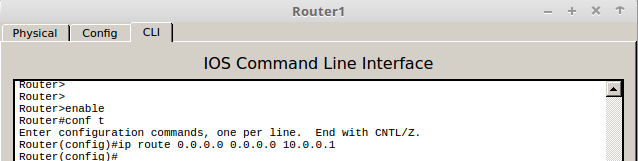
\includegraphics[width=\textwidth]{5routerdefgw}
    \caption{Configuring static routes for routers}
    \label{fig:5routerdefgw}
\end{subfigure}
%
\begin{subfigure}{0.5\textwidth}
 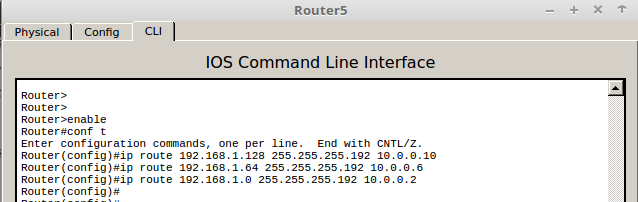
\includegraphics[width=\textwidth]{5router5def}
    \caption{Configuring static route for Router5}
    \label{fig:5router5def}
\end{subfigure}

\end{figure}

\begin{figure}[h]
    \centering
    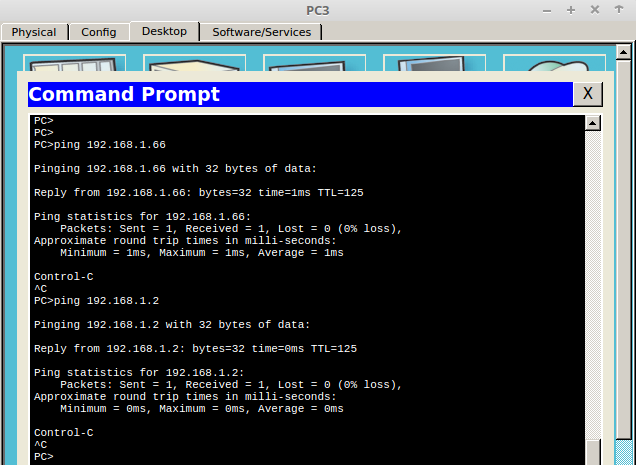
\includegraphics[scale=0.3]{5pingtest}
    \caption{Checking reachability between h}
    \label{fig:5pingtest}
\end{figure}

After the default routes are set we can check the connectivity by pinging the hosts. As seen in Figure \ref{fig:5pingtest}, we have full connection.

\subsection{Routing with RIP}

Now removing the static routes from the routers. And trying to configure the RIP routing protocol, we cannot assign the networks subnet mask. This is because RIP version 1 is used as default routing protocol and RIP version 1 only supports classfull routing so it only takes an IP address. If we give the IP address 192.168.1.128 it automatically assumes its in the network 192.168.1.0, which is not possible with our classless topology. Therefore we do not have reachability between the different nodes. If we had configured the topology using OSPF then there would be complete reachability between the different nodes as OSPF supports classless routing. 

\section{Spanning-Tree protocol in Packet Tracer}

Implementing the topology shown in Figure \ref{fig:6topassign} using the generic switches and connecting them using the crossover copper cable. Then we assign the switch priority number by going to the \textit{config mode} and using the command \textbf{spanning-tree vlan 1 priority {\textless}Bid{\textgreater}} where Bid is given in Figure \ref{fig:6topassign}. 

\begin{figure}[h]
    \centering
    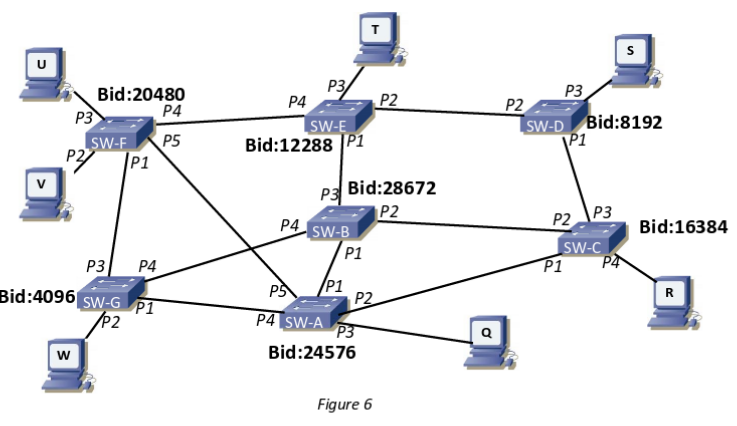
\includegraphics[scale=0.3]{6topassign}
    \caption{Topology from Figure 6 in Assignment 7. }
    \label{fig:6topassign}
\end{figure}

\begin{figure}[h]
    \centering
    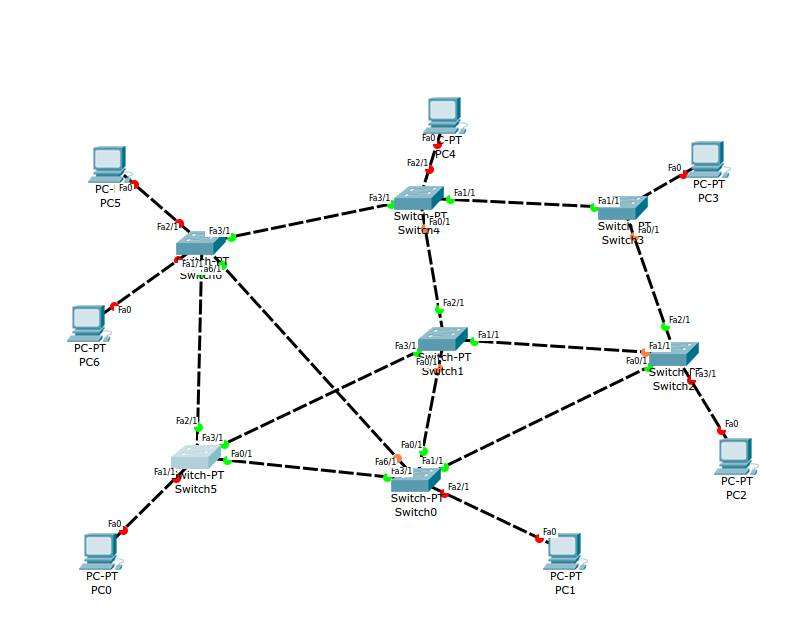
\includegraphics[scale=0.2]{6top}
    \caption{The topology of \ref{fig:6topassign} in PacketTracer}
    \label{fig:6top}
\end{figure}

The topology in the PacketTracer can be seen in Figure \ref{fig:6top}.Then after we have created the topology we can check the port roles/status of the switches using the command \textbf{show spanning-tree} in \textit{enable mode}. We can see the port status in Table \ref{tab:6portstatus} where D is Designated port, R is the Root port and U is Blocked port. 

\begin{table}[h]
 \centering
    \begin{tabular}{|c|c|c|c|c|c|}
    \hline
         & p0 & p1 & p2 & p3 & p4 \\
    \hline
    Switch-A & D & D & D & R & U \\
    Switch-B & U & D & D & R & - \\
    Switch-C & R & U & D & D & - \\
    Switch-D & U & R & D & - & - \\
    Switch-E & U & D & D & R & - \\
    Switch-F & R & D & D & D & D \\
    Switch-G & D & D & D & D & - \\
    \hline
    \end{tabular}
    \caption{Port roles for the Figure \ref{fig:6top} topology}
    \label{tab:6portstatus}
\end{table}

\end{document}
